\documentclass[runningheads,a4paper]{llncs}

%\usepackage[spanish]{babel}
\usepackage{amssymb}
\setcounter{tocdepth}{3}
\usepackage{graphicx}

\usepackage{color}
\usepackage{listings}
\definecolor{mygreen}{rgb}{0,0.6,0}
\lstdefinestyle{python}{language=[Python],  rulecolor=\color{blue!80!black}}
\lstset{language = csh, language = python, basicstyle = \bfseries\ttfamily, keywordstyle = \color{blue}, commentstyle=\color{mygreen}, breaklines = true, showstringspaces=false}
\usepackage{xcolor, pstricks}
\usepackage{multicol}

\usepackage[spanish]{babel}
\usepackage[pdftex]{hyperref}

\usepackage{url}
\urldef{\mailsa}\path|{amalia.ibarra, gabriela.martinez}@estudiantes.matcom.uh.cu|      
\newcommand{\keywords}[1]{\par\addvspace\baselineskip
\noindent\keywordname\enspace\ignorespaces#1}


\begin{document}
\renewcommand{\abstractname}{Resumen.}
\renewcommand{\keywordname}{\textbf{Palabras Clave:}}
\renewcommand{\refname}{Referencias}
\renewcommand{\tablename}{Tabla}

\mainmatter  % start of an individual contribution

\title{Proyecto de Prolog.\\Juego Hive.}

\titlerunning{Prolog-Hive}

\author{Amalia Ibarra Rodr\'iguez\\
	Gabriela B. Mart\'inez Giraldo}

\authorrunning{Amalia et al.}

\institute{Universidad de La Habana,\\La Habana, Cuba\\
Grupo C-412\\
\mailsa\\}
\maketitle


\section{Descripci\'on del problema}\label{sec:ex1}

El presente proyecto pretende ofrecer una impletenci\'on del juego Hive en el lenguaje de programaci\'on Prolog. Este es un juego de mesa muy curioso, en el cual cada jugador cuenta con 11 piezas que representan diferentes insectos a escoger entre: \emph{abeja reina}(1), \emph{hormiga}(3), \emph{ara\~na}(2), \emph{escarabajo}(2), \emph{bicho bola}(1), \emph{mariquita}(1), \emph{mosquito}(1) y \emph{saltamontes}(3).

A continuaci\'on se presentan las ideas seguidas para modelar las situaciones requeridas por dicho juego.




\section{Consideraciones sobre la disposici\'on del tablero}

En Hive no existe un tablero fijo, sino que se va expandiendo a medida que avanza el juego. Este est\'a conformado por casillas hexagonales que pueden ser ocupadas por los insectos. A partir de que se coloca el primero, el tablero va creciendo  a su alrederor. Se asume que la primera baldosa que aparece en el juego es la 0,0 y a partir de ella se definen sus adyacentes como:

(r-1, c)

(r, c-1)

(r+1, c-1)

(r+1, c)

(r, c+1)

(r-1, c+1)

si se consideran siguiendo el sentido de las manecillas del reloj y empezando por la casilla superior izquierda.\\[20cm]

De esta forma, un tablero ir\'ia quedando como:

\begin{figure}
	\centering
	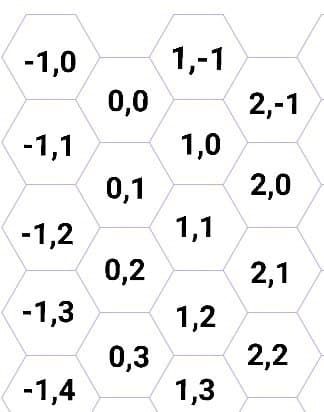
\includegraphics[width = 4cm]{images/board}
	\caption{Coordenadas del tablero}\label{fig:lcc1}
\end{figure}

\section{C\'omo correr el proyecto}
En una consola dentro de la carpeta /src:
\begin{enumerate}
	\item Ejecutar el comando swipl main.pl 
	\item Una vez en el entorno de swipl ejecutar start().
\end{enumerate} 

Este \'ultimo inicializa los predicados que mantienen el estado de la partida. A partir de este punto comienza el juego y se pueden insertar y mover fichas a trav\'es de lo predicados:

\begin{enumerate}
	\item insert\_to(Bug). 
	
	Aqu\'i solo es necesario el nombre del insecto (que se especifica en Bug) pues se utiliza para insertar la primera ficha del juego que por defecto se ubica en (0,0).\\
	
	\item insert\_to(Bug, X, Y). 
	
	Inserta el insecto (Bug) en la posici\'on (X, Y).\\
	
	\item move\_to(X1, Y1, X2, Y2).
	
	 Mueve la ficha ubicada en (X1, Y1) hacia la posici\'on (X2, Y2).\\
	
	\item move\_to(X1, Y1, X2, Y2, X3, Y3). 
	
	El bicho bola en la posici\'on (X1, Y1) mueve la ficha ubicada en (X2, Y2) hacia la posici\'on (X3, Y3).\\
	
	\item move\_to(X1, Y1, X2, Y2, X3, Y3). 
	
	El mosquito ubicado en (X1, Y1) se mueve hacia (X3, Y3) usando el poder del insecto qu ese halla en (X2, Y2).\\
	
	\item move\_to(X1, Y1, X2, Y2, X3, Y3, X4, Y4). 
	
	El mosquito en la posici\'on  (X1, Y1) utiliza el poder del bicho bola en (X2, Y2) para mover la ficha en (X3, Y3) hacia la posici\'on (X4, Y4).\\
\end{enumerate}

Dichos predicados actualizar\'an el estado del juego y evaluar\'an \emph{true} en caso de ejecutar un movimiento v\'alido o \emph{false} en el caso contrario. Los insectos que se aceptan como entrada son: \emph{queen, spider, ant, ladybug, pillbug, mosquito, grasshopper} y \emph{beetle}.


\section{Aspectos claves de la implementaci\'on}
Para tener control del estado del juego fue necesario definir un n\'umero de predicados din\'amicos que llevaran el conocimiento de la situaci\'on. 

As\'i se define una ficha en una posici\'on dada seg\'un el predicado \emph{tile(Bug, Colour, X, Y, Level)}, donde \emph{Bug} es el nombre del insecto, \emph{Colour} su color, \emph{X} y \emph{Y} sus coordenadas en el tablero y \emph{Level} su nivel. Este \'ultimo valor se utiliza para representar la existencia de fichas apiladas (recordemos que el escarabajo es capaz de subir encima de otros insectos). 

Se tiene constancia adem\'as de la cantidad de movimientos efectuados durante el juego a trav\'es de \emph{move\_count/1}, el cual determina qu\'e turno corresponde a cada jugador, considerando que las blancas son las primeras en jugar.

Para limitar el n\'umero de insectos de cada tipo se defini\'o el predicado \emph{max\_count/2}, el cual recibe el nombre de una especie espec\'ifica y retorna la cantidad m\'axima que se pueden insertar. A su vez la cantidad de fichas de cada tipo colocadas en el tablero por cada jugador se registran a partir del predicado \emph{insertion\_count/2}.

\subsection{Movimientos de cada insecto}

En general ning\'un insecto puede ser insertado en una posici\'on ocupada del tablero, ni en una donde colinde con fichas de color contrario. Tampoco puede a\~nadirse a una casilla fuera de la colmena. Estas comprobaciones se llevan a trav\'es de los predicados \emph{position\_available/2},\emph{validate\_insertion/4} que reciben los detalles necesarios del insecto a insertar.

Las reglas exigen insertar la \emph{abeja reina} antes del 4to turno, y detallan que no es posible mover ninguna pieza antes de que esta est\'e en juego. Con este fin se hizo uso del predicado \emph{queen\_in\_game/1} que no hace m\'as que consultar en la BD de prolog la existencia de una reina de un color dado antes de mover cualquier insecto. 

Como cada insecto tiene sus particularidades a la hora de moverse fue necesario implementar un predicado espec\'ifico para cada uno, dado que s\'olo se comparten pocas especificaciones como la de no tener otro insecto encima en ese momento y la de no romper la colmena. Estas se llevan con los predicados \emph{pilled/2} y \emph{one\_hive\_rule\_fullfill/5}. Analicemos un poco m\'as de cerca qu\'e estrategia se sigui\'o para verificar los movimientos v\'alidos, definidos en su mayor\'ia en el archivo \emph{moves.pl}:

\begin{enumerate}
	\item \emph{Queen bee}: La abeja reina s\'olo da un paso en cada turno, por lo que para validar una candidata  a pr\'oxima posici\'on s\'olo se requiere definir las direcciones hacia las que se encuentran las celdas adyacentes y comprobar que la candidata sea una de estas y est\'e disponible. Como parte de los requerimientos generales se debe comprobar tambi\'en que no exista un puente que bloquee este paso, lo cual nos facilita el predicado \emph{not\_blocked/5}.
	
	\item \emph{Beetle}: Su movimiento es similar al de la reina, s\'olo se omite la comprobaci\'on de que la celda est\'e disponible, dado que el poder especial de este insecto es precisamente saltar sobre otros.
	
	\item \emph{Pillbug}: Puede moverse un \'unico paso hasta posiciones libres, completamente igual a la reina. En este se a\~nade un predicado extra que permita al pillbug hacer uso de su poder, mover fichas adyacentes. Para ello se considera que no pueden existir puentes entre el primer insecto adyacente y el bicho bola ni entre este \'ultimo y la posici\'on destino.
	
	\item \emph{Ant}: La hormiga puede hacer recorridos m\'as largos alrededor de la colmena, topando siempre con celdas ocupadas. La forma de comprobar la existencia de dicho camino entre un origen y un destino dado fue a trav\'es de un BFS o recorrido primero en anchura como se muestra a continuaci\'on, comprobando que no existan puentes que bloqueen su paso.
	
	\begin{center}
		\begin{lstlisting}
  bfsft(Source, Destination):- 
     bfsfta([Source], [Source], Destination).
  bfsfta([[X,Y]|_R], _Seen, [X, Y]).

  bfsfta([[X,Y]|R], Seen, [Xd, Yd]):- 
     bagof([X2, Y2],
     (free_adj_tile((X,Y),(X2, Y2)),
     not_blocked(X, Y, X2, Y2, _Bridges), 
     not(member([X2,Y2], Seen))), Adj),
     append(Seen, Adj, UpdSeen), 
     append(R, Adj, UpdR), !,
     bfsfta(UpdR, UpdSeen, [Xd, Yd]);
     bfsfta(R, Seen, [Xd, Yd]).
		\end{lstlisting}
	\end{center} 
	
	\item \emph{Spider}: Similar al caso anterior, su recorrido es bordeando la colmena, s\'olo que est\'a limitao a una cantidad de 3 casillas en total, por lo que se utiliza una modificaci\'on del predicado anterior.
	
	\item \emph{Lady Bug}: De igual forma la mariquita requiere de un m\'etodo para comprobar la existencia de un camino de tama\~no 3 entre dos casillas dadas, s\'olo que en este caso las dos primeras deben ser sobre baldosas ocupadas por otros insectos y la \'ultima una libre. Esta no requiere la comprobaci\'on de si existen puentes en el camino, dado que su ventaja es precisamente el entrar y salir de posiciones bloqueadas.
	
	\item \emph{Grasshopper}: El saltamontes puede saltar por un grupo de insectos que se encuentren dispuestos en l\'inea recta en cualquier direcci\'on, horizontal o vetical. Con \emph{validate\_grasshoper\_move/4} se verifica que exista un camino que cumpla las condiciones anteriores, consultando la direcci\'on y sentido del movimiento que se pretende efectuar y validando luego que exista en cada paso de ese camino un insecto en el tablero.
	
	\item \emph{Mosquito}: El mosquito es una pieza bastante vers\'atil, pues puede adquirir el poder de cualquier otra ficha en juego que se encuentre adyacente a \'el. A su vez, cuando se haya logrado el comportamiento correcto del resto de los insectos este se hace bastante sencillo, dado que s\'olo requiere replicar el comportamiento de las mismas.
	
\end{enumerate}

\end{document}
